\documentclass{article}
\usepackage[utf8]{inputenc}
\usepackage[a4paper, total={6.5in, 10in}]{geometry}
\usepackage{merriweather}
\usepackage[hidelinks]{hyperref}
\usepackage{graphicx}
\usepackage{xcolor}

% for markdown inline code effect
\definecolor{bgcolor}{HTML}{E0E0E0}
\let\oldtexttt\texttt
\renewcommand{\texttt}[1]{
  \colorbox{bgcolor}{\oldtexttt{#1}}
  }

\title{\textbf{
CS311 Report \\ 
Assignment 0 - Simulation Using Java
}}
\author{
  B Siddharth Prabhu\\
  \href{mailto:200010003@iitdh.ac.in}{\texttt{200010003@iitdh.ac.in}}
  \and
  Devdatt N\\
  \href{mailto:200010012@iitdh.ac.in}{\texttt{200010012@iitdh.ac.in}}
  }
  
\date{9 August 2022}

\begin{document}

\maketitle

\section{Introduction}
Here we attempt to calculate the approximate time an infiltrator would take to cross a border into a defending country. The border, embedded with probability governed sensors pose a challenge to the infiltrator. Therefore, we must take an algorithmic approach to the problem by varying the probability and width parameters. 
% v brief idea abt stuff, pls do this ty !!!

\section{Assumptions \& Considerations}
Different elements of the scenario have been modeled as classes, included in the same folder as our main program, \texttt{Main.java}. Below are the assumptions and considerations we've taken into account during the coding process:

\subsection{Border}
The border between the AC and DC consists of a rectangular (discretized) grid of sensor cells, which has infinite length, and width $W$. We consider the initial position of an infiltrator to be one of the cells in the first layer of the border. (Considering it to be outside the border at $t=0$ would just translate the generated graph, and wouldn't change the trends.)

\begin{figure}[hbt]
    \centering
    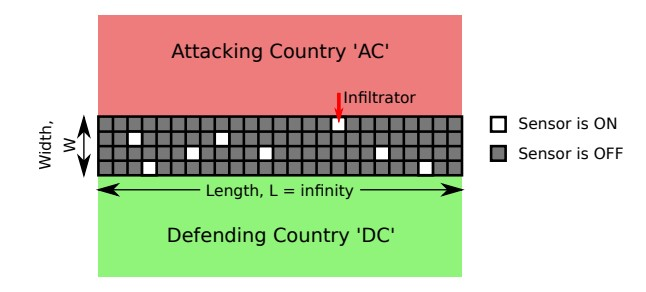
\includegraphics{border-img.jpg}
    \caption{Illustration of the scenario}
    \label{fig:border-img}
\end{figure}

\subsection{Sensors and Infiltrator}
The infiltrator is initially placed on a sensor at depth zero. (The terms `width' and `depth' are used interchangeably here.) Each sensor is ON or OFF based on a probability `p' (0 \textless~p \textless~1).
Things to consider include:
\begin{enumerate}
    \item Moving left or right has no payoff, since L is infinity and the sensor states are all based on a probability value that's independent of the decisions of other sensors.
    \item Moving upwards would be counteractive to crossing the border. It would be better to stop and wait at the current sensor until a favourable scenario exists (such that the current sensor is off AND one of the three adjacent sensors of the next level is also off.
\end{enumerate}

An initial approach would be to render the states of only the 8 `visible' sensors, that are reachable from the current cell. This is already a significant reduction from having to render the entire $L \times W$ grid. However, we can do better. Since we only ever move forward, we can just simulate the current cell, `W', and the three `forward' cells, which we call `A', `S', and `D', due to their QWERTY intuitiveness. At the final layer, only 1 cell (`W') has to be generated. Also, the infiltrator itself keeps track of the extent to which it has crossed the border, as a class attribute.

\begin{figure}[hbt]
    \centering
    \includegraphics[scale=0.4275]{evolgraph.png}
    \caption{Evolution of our approach}
    \label{fig:evolve}
\end{figure}

\subsection{Environment Variables}

\begin{itemize}
    \item \texttt{p\_arr} and \texttt{width\_arr} contain different values of `p' and `W' respectively, that we loop over to obtain different values for infiltration time `t'.
    \item \texttt{num\_trials} is responsible for the number of trials done for each $(p,W)$ pair. However (in its current form), the Java and Python programs don't communicate with each other. So, the .py program is set up for \texttt{num\_trials = 5}
    \item The \texttt{Clock} class handles time-tracking for each trial of the experiment. 
    \item The averages over the trials are calculated in the Python file, and are then processed to plot the required graph.
\end{itemize}

\section{Code Compilation and Execution} 
To get started, we check if java is available using \texttt{java -version} from the command line.
\\\\We use the following command line arguments to run and test our program : 
\begin{enumerate}
    \item  \texttt{javac *.java}
    \item  \texttt{java Main}
    \item  \texttt{python3 graphplot.py}
\end{enumerate}
As an alternative, we have also included a bash script which executes all the arguments which can be run with the command line argument \texttt{bash run.sh}.
\\\\In our program's case, separate inputs for widths and p don't have to be entered since all combinations are stored within arrays within. Output is configured to be saved in the \texttt{output.txt} file where each line is in the format (p,w,t) where `p', `W' are parameters, and `t' is time taken.
\\\\We have used WSL(Windows Subsystem for Linux) to emulate a Linux environment, so to open the generated graph from the WSL command line we use \texttt{wslview graph.png}.

% sir recompile and look at the code parts lol
\section{Graphical Representation}

We have generated a three dimensional graph with p, width and time on the x,y and z axes respectively using matplotlib. The obtained graph is as below:
\begin{figure}[hbt]
    \centering
    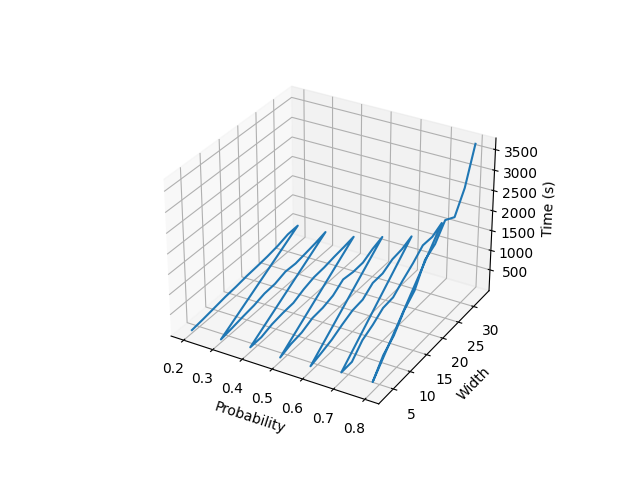
\includegraphics[scale=0.9]{graph.png}
    \caption{Variation of time with p,w combinations}
    \label{fig:graphfinal}
\end{figure}

% graph
% some words abt it idk

\section{Observations}

As we can see, average time to cross the border increases as probability `p' of the sensor switching on and width increases. For a uniform `p', as width increases the rate of change of time taken to cross the border remains largely the same. 
\\\\However, at high widths and changing `p', the differential of time taken with respect to width can be seen as more exponential. This is to be expected since it is almost impossible to cross the border as `p' approaches 1. 
% things about effect of w on t, 
% also p on t

\section{Conclusion}

Apart from a rather strange downward slant around \texttt{width = 30} and \texttt{p = 0.8}, the graph remains as expected with time to cross the border increasing along with (p,w) increasing. This might be because true randomness is hard to achieve and even though we have tested each combination five times, we need a higher number of trials to have an effect of choosing a truly random number. 
\\\\Nevertheless, we have managed to deliver a rather optimal algorithm to generate the time taken by ignoring the unfruitful left and right moves.
% sir what is that sentence
% i mean it's 100% true
\end{document}
% great work piro